\documentclass{article}

% packages
\usepackage{amsmath, amsthm, thmtools, amsfonts, amssymb, luacode, catchfile, tikzducks, hyperref, ifthen}
\ifcsname c@kobocompile\endcsname
	\usepackage[a5paper, total={1072pt, 1448pt}, margin=10pt, includeheadfoot]{geometry} % set page margins
\else
	\usepackage[a4paper, margin=50pt, includeheadfoot]{geometry}
\fi
\usepackage[shortlabels]{enumitem}
\usepackage[skip=3pt, indent=0pt]{parskip}

% language
\usepackage[bidi=basic, layout=tabular, provide=*]{babel}
\ifcsname c@english\endcsname
	\babelprovide[main, import]{english}
\else
	\babelprovide[main, import]{hebrew}
	\babelprovide{rl}
\fi
%\babelfont{rm}{Libertinus Serif}
\babelfont{rm}[Renderer=Harfbuzz]{Libertinus Serif}
\babelfont{sf}{Libertinus Sans}
\babelfont{tt}{Libertinus Mono}

% style
\AddToHook{cmd/section/before}{\clearpage}	% Add line break before section
\linespread{1.3}
\setcounter{secnumdepth}{0}		% Remove default number tags from sections, this won't do well with theorems
\AtBeginDocument{\setlength{\belowdisplayskip}{3pt}}
\AtBeginDocument{\setlength{\abovedisplayskip}{3pt}}
\graphicspath{ {../images/} }

% operators
\DeclareMathOperator\cis{cis}
\DeclareMathOperator\Sp{Sp}
\DeclareMathOperator\tr{tr}
\DeclareMathOperator\im{Im}
\DeclareMathOperator\re{Re}
\DeclareMathOperator\diag{diag}
\DeclareMathOperator*\lowlim{\underline{lim}}
\DeclareMathOperator*\uplim{\overline{lim}}
\DeclareMathOperator\rng{rng}
\DeclareMathOperator\Sym{Sym}
\DeclareMathOperator\Arg{Arg}
\DeclareMathOperator\Log{Log}
\DeclareMathOperator\dom{dom}
\DeclareMathOperator\supp{Supp}
\DeclareMathOperator\var{Var}
\DeclareMathOperator\cov{Cov}

% commands
%\renewcommand\qedsymbol{\textbf{מש''ל}}
%\renewcommand\qedsymbol{\fbox{\emoji{lizard}}}
\newcommand{\Aa}[0]{\mathcal{A}}
\newcommand{\Bb}[0]{\mathcal{B}}
\newcommand{\CC}[0]{\mathbb{C}}
\newcommand{\Cc}[0]{\mathcal{C}}
\newcommand{\EE}[0]{\mathbb{E}}
\newcommand{\FF}[0]{\mathbb{F}}
\newcommand{\Ff}[0]{\mathcal{F}}
\newcommand{\Ii}[0]{\mathcal{I}}
\newcommand{\Gg}[0]{\mathcal{G}}
\newcommand{\Ll}[0]{\mathcal{L}}
\newcommand{\Mm}[0]{\mathcal{M}}
\newcommand{\NN}[0]{\mathbb{N}}
\newcommand{\Nn}[0]{\mathcal{N}}
\newcommand{\PP}[0]{\mathbb{P}}
\newcommand{\Pp}[0]{\mathcal{P}}
\newcommand{\QQ}[0]{\mathbb{Q}}
\newcommand{\RR}[0]{\mathbb{R}}
\newcommand{\Rr}[0]{\mathcal{R}}
\newcommand{\Ss}[0]{\mathcal{S}}
\newcommand{\TT}[0]{\mathbb{T}}
\newcommand{\Uu}[0]{\mathcal{U}}
\newcommand{\Vv}[0]{\mathcal{V}}
\newcommand{\Ww}[0]{\mathcal{W}}
\newcommand{\ZZ}[0]{\mathbb{Z}}
\newcommand{\acts}[0]{\circlearrowright}
\newcommand{\explain}[2] {
	\begin{flalign*}
		 && \text{#2} && \text{#1}
	\end{flalign*}
}
\newcommand{\maketitleprint}[0]{ \begin{center}
	%\begin{tikzpicture}[scale=3]
	%	\duck[graduate=gray!20!black, tassel=red!70!black]
	%\end{tikzpicture}	
	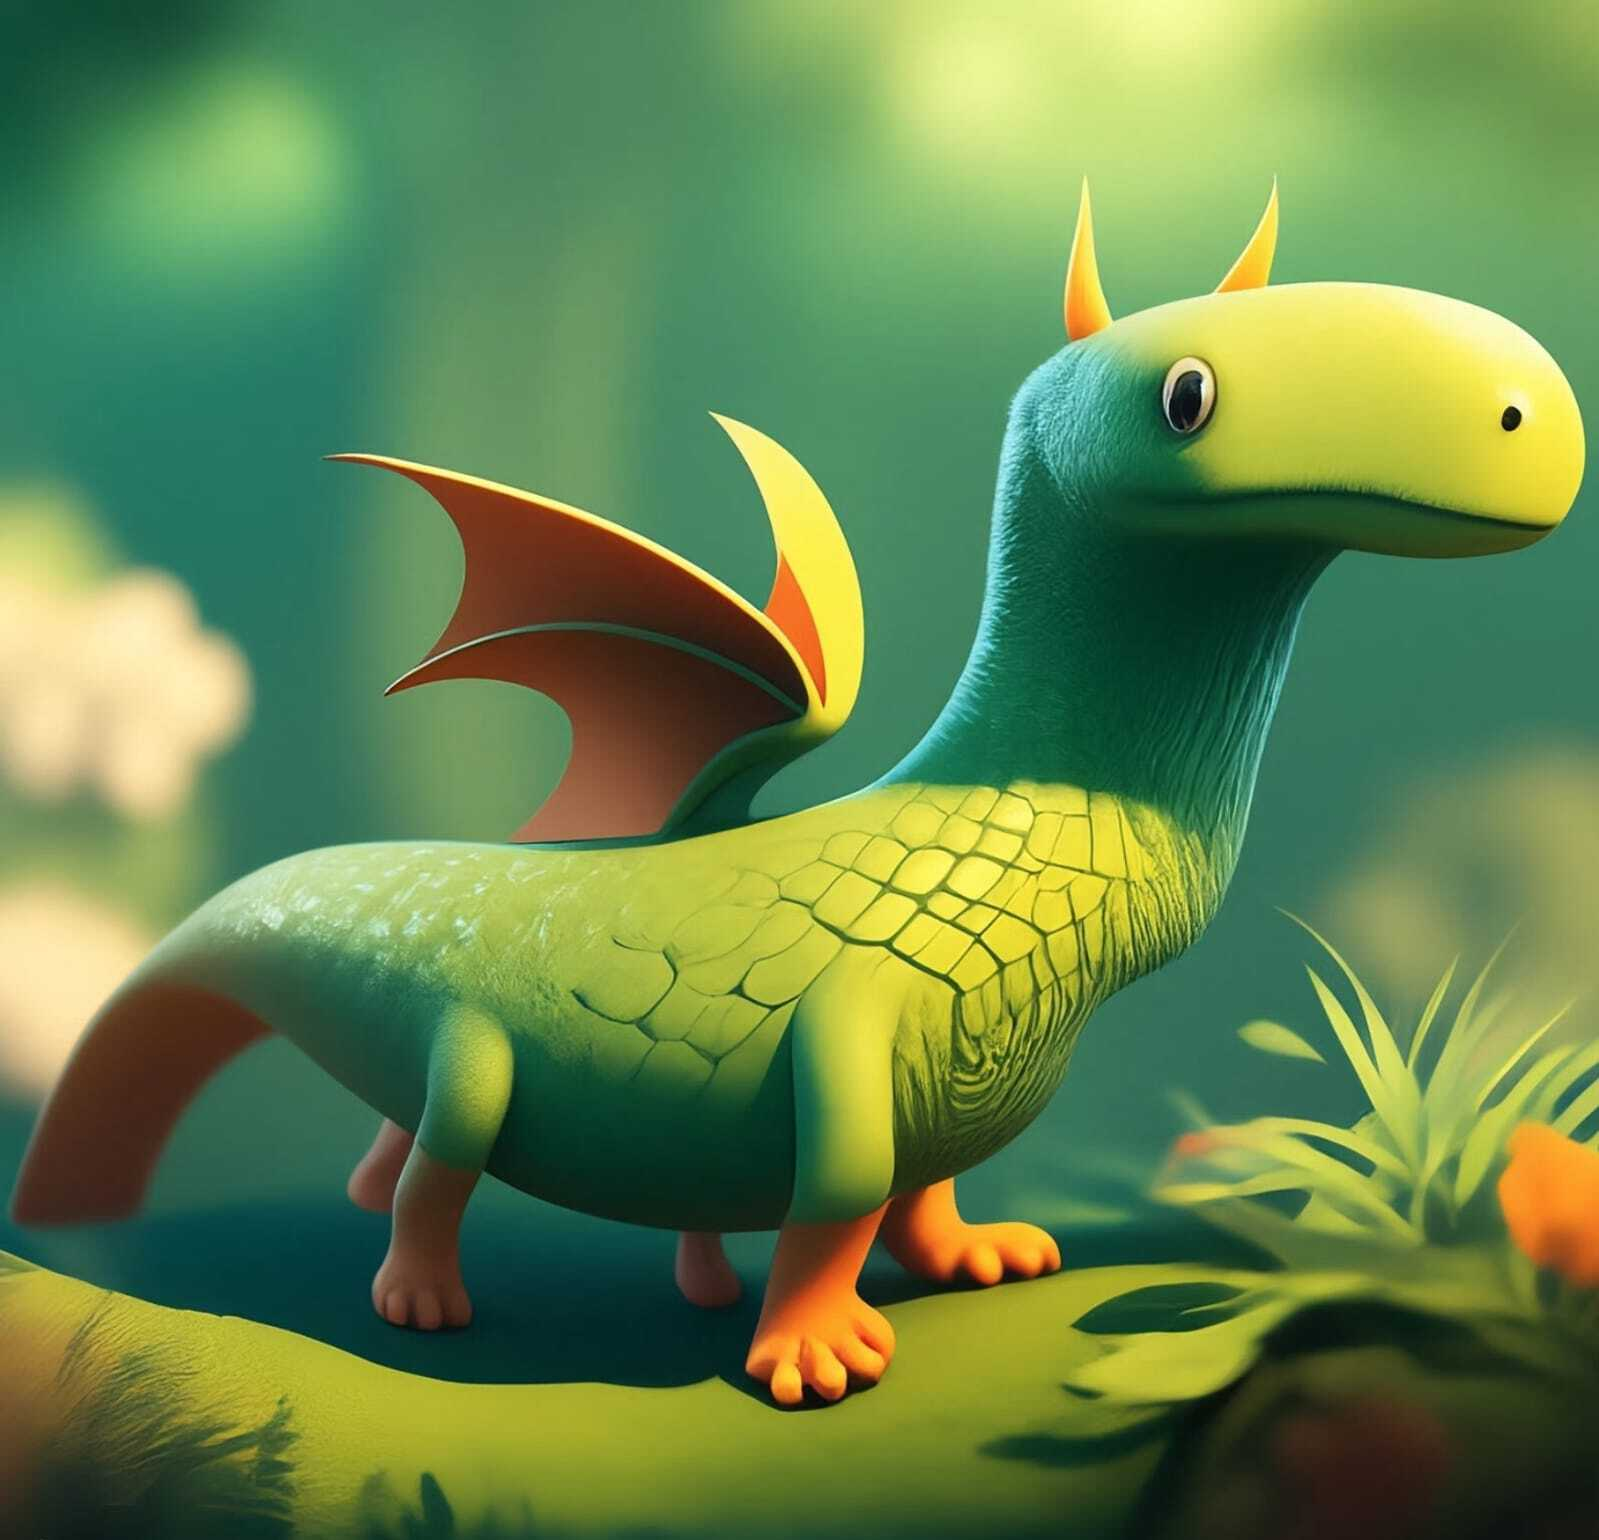
\includegraphics[width=6cm]{cover}
\end{center}
}

% theorem commands
\newtheoremstyle{c_remark}
	{}	% Space above
	{}	% Space below
	{}% Body font
	{}	% Indent amount
	{\bfseries}	% Theorem head font
	{}	% Punctuation after theorem head
	{.5em}	% Space after theorem head
	{\thmname{#1}\thmnumber{ #2}\thmnote{ \normalfont{\text{(#3)}}}}	% head content
\newtheoremstyle{c_definition}
	{3pt}	% Space above
	{3pt}	% Space below
	{}% Body font
	{}	% Indent amount
	{\bfseries}	% Theorem head font
	{}	% Punctuation after theorem head
	{.5em}	% Space after theorem head
	{\thmname{#1}\thmnumber{ #2}\thmnote{ \normalfont{\text{(#3)}}}}	% head content
\newtheoremstyle{c_plain}
	{3pt}	% Space above
	{3pt}	% Space below
	{\itshape}% Body font
	{}	% Indent amount
	{\bfseries}	% Theorem head font
	{}	% Punctuation after theorem head
	{.5em}	% Space after theorem head
	{\thmname{#1}\thmnumber{ #2}\thmnote{ \text{(#3)}}}	% head content

\ifcsname c@english\endcsname
	\theoremstyle{plain}
	\newtheorem{theorem}{Theorem}[section]
	\newtheorem{lemma}[theorem]{Lemma}
	\newtheorem{proposition}[theorem]{Proposition}
	\newtheorem*{proposition*}{Proposition}
	%\newtheorem{corollary}[theorem]{אין חלופה עברית}

	\theoremstyle{definition}
	\newtheorem{definition}[theorem]{Definition}
	\newtheorem*{definition*}{Definition}
	\newtheorem{example}{Example}[section]
	\newtheorem{exercise}{Exercise}[section]

	\theoremstyle{remark}
	\newtheorem*{remark}{Remark}
	\newtheorem*{solution}{Solution}
	\newtheorem{conclusion}[theorem]{Conclusion}
	\newtheorem{notation}[theorem]{Notation}
\else
	\theoremstyle{c_plain}
	\newtheorem{theorem}{משפט}[section]
	\newtheorem{lemma}[theorem]{למה}
	\newtheorem{proposition}[theorem]{טענה}
	\newtheorem*{proposition*}{טענה}
	%\newtheorem{corollary}[theorem]{אין חלופה עברית}

	\theoremstyle{c_definition}
	\newtheorem{definition}[theorem]{הגדרה}
	\newtheorem*{definition*}{הגדרה}
	\newtheorem{example}{דוגמה}[section]
	\newtheorem{exercise}{תרגיל}[section]

	\theoremstyle{c_remark}
	\newtheorem*{remark}{הערה}
	\newtheorem*{solution}{פתרון}
	\newtheorem{conclusion}[theorem]{מסקנה}
	\newtheorem{notation}[theorem]{סימון}
\fi

% Questions related commands
\newcounter{question}
\setcounter{question}{1}
\newcounter{sub_question}
\setcounter{sub_question}{1}

\ifcsname c@english\endcsname
	\newcommand{\question}[1][0]{
		\ifthenelse{#1 = 0}{}{\setcounter{question}{#1}}
		\section{Question \arabic{question}}
		\addtocounter{question}{1}
		\setcounter{sub_question}{1}
	}

	\newcommand{\subquestion}[1][0]{
		\ifthenelse{#1 = 0}{}{\setcounter{sub_question}{#1}}
		\subsection{Part \alph{sub_question}}
		\addtocounter{sub_question}{1}
	}
\else
	\newcommand{\question}[1][0]{
		\ifthenelse{#1 = 0}{}{\setcounter{question}{#1}}
		\section{שאלה \arabic{question}}
		\addtocounter{question}{1}
		\setcounter{sub_question}{1}
	}

	\newcommand{\subquestion}[1][0]{
		\ifthenelse{#1 = 0}{}{\setcounter{sub_question}{#1}}
		\subsection{סעיף \localecounter{letters.gershayim}{sub_question}}
		\addtocounter{sub_question}{1}
	}
\fi

% import lua and start of document
\directlua{common = require ('../common')}

\GetEnv{AUTHOR}

% headers
\author{\AUTHOR}
\date\today

\title{פתרון מטלה 11 --- מבוא ללוגיקה, 80423}

\begin{document}
\maketitle
\maketitleprint{}

\question{}
\subquestion{}
נשלים את הוכחת טענת ההלוך־ושוב מהתרגול על־ידי הוכחה שההעתקה שנבנתה היא איזומורפיזם של מבנים בשפה $L$.
\begin{proof}
	נבחין שהשפה $L$ מורכבת מסימני יחס בלבד, לכן מספיק לבדוק ש־$f : \Mm \to \Nn$ היא חד־חד ערכית, על ומשמרת סימני יחס בלבד.
	נבדוק אם $f$ חד־חד ערכית.
	יהיו $x, y \in M$, אז קיימים $n, m$ כך ש־$f(x) = f_n(x), f(y) = f_m(y)$, ללא הגבלת הכלליות נניח $m < n$ ולכן בהכרח גם $f(y) = f_n(y)$, אבל ידוע גם ש־$f_n$ חד־חד ערכית, ולכן $f(x) = f_n(x) \ne f_n(y) = f(y)$ ומצאנו חד־חד ערכיות.
	ראינו בתרגול ש־$f$ על, ולכן מספיק שנבדוק אם היא משמרת יחסים (שכן אין בשפה עוד מלבד יחסים).
	נניח $R \in \operatorname{Rel}_{L, n}$ עבור $n \in \NN$, וכן $x_0, \dots, x_{n - 1} \in M$, אז מסופיות הקבוצה קיים גם $m \in \NN$ כך ש־$f(x_i) = f_m(x_i)$ לכל $i < n$.
	כמובן נובע
	\[
		f(R^\Mm(x_0, \dots, x_{n - 1}))
		= f_n(R^\Mm(x_0, \dots, x_{n - 1}))
		= R^\Nn(f_n(x_0), \dots, f_n(x_{n - 1}))
		= R^\Nn(f(x_0), \dots, f(x_{n - 1}))
	\]
	ומצאנו שאכן $f$ היא איזומורפיזם המרחיב את $g$.
\end{proof}

\subquestion{}
נניח ש־$\Aa$ ו־$\Bb$ מבנים בני־מניה ל־$L_=$. \\
נראה שיש $A_0 \subseteq A, B_0 \subseteq B$ ואיזומורפיזם $f : \langle A_0 \rangle \to \langle B_0 \rangle$ שאינו ניתן להרחבה לאיזומורפיזם $g : \Aa \to \Bb$.
\begin{proof}
	נוריד כמות סופית של איברים מ־$A$ כדי להגדיר את $A_0$, נבחין שאכן יש לנו יכולת לעשות זאת (והיא לא מצריכה בחירה).
	אנו יודעים ש־$|A| = \aleph_0$ ולכן אם $A_0 \subseteq A$ כך ש־$|A \setminus A_0| < \aleph_0$ אז $|A_0| = \aleph_0$ ובהתאם קיימת פונקציה חד־חד ערכית ועל $f : A_0 \to B$.
	נבחין שכתוצאה ישירה מאקסיומת ההיקפיות הפונקציה שהגדרנו מקיימת,
	\[
		\forall x, y \in A,
		\quad
		f(x =^\Aa y)
		= f(x) =^\Bb f(y)
	\]
	לכן $f : \Aa \to \Bb$ איזומורפיזם.

	עתה נניח בשלילה ש־$g$ איזומורפיזם המרחיב את $f$.
	נבחר $x \in A \setminus A_0$, אכן קיים כזה מההגדרה שלנו.
	אם נניח ש־$f(x) = x' \in B$, נקבל שקיים $y \in A_0$ כך ש־$g(y) = f(y) = x'$.
	לכן מחד־חד ערכיות נובע $x = y$, ובהתאם $x \in A_0 \cap (A \setminus A_0) = \emptyset$, סתירה.
\end{proof}

\question{}
\subquestion{}
תהי $L = \{ < \}$ שפה עם יחס דו־מקומי, נסמן ב־$T_0$ את התורה שגורסת כי $<$ יחס אנטי־רפלקסיבי, טרנזיטיבי וקווי. \\
נניח ש־$A, B$ קבוצות כך ש־$\Aa, \Bb \models T_0$ וגם $|\Aa| = A, |\Bb| = B$. \\
נראה שאם $f : A \to B$ חד־חד ערכית ועל היא איזומורפיזם $\Aa \to \Bb$ אם ורק אם לכל $a_0, a_1 \in A$ כך ש־$a_0 <^\Aa a_1$ מתקיים גם $f(a_0) <^\Bb f(a_1)$.
\begin{proof}
	נניח ש־$f$ איזומורפיזם, לכן נובע מהגדרה $a_0 <^\Aa a_1 \iff f(a_0) <^\Bb f(a_1)$ וסיימנו.

	נניח את הכיוון השני, ונראה ש־$f$ היא אכן איזומורפיזם.
	נבחין כי בשפה אין קבועים או סימני פונקציה, לכן כל שם עצם יהיה משתנה, אז לכל הצבה שהיא מהנתון נקבל ש־$f$ משמרת שמות עצם כפי שרצינו.
	נבחין כי כל נוסחה יסודית היא מהצורה $x < y$, ולכן לכל הצבה מההנחה הפונקציה משמרת יחסים, ולכן $f$ עומדת בהגדרה של איזומורפיזם.
\end{proof}

\subquestion{}
נניח ש־$\Mm, \Nn$ מודלים של $T_0$, וכן
\[
	A = \{ a_0, \dots, a_{k - 1} \} \subseteq M,
	\quad
	B = \{ b_0, \dots, b_{k - 1} \} \subseteq N
\]
כך ש־$a_0 <^\Mm \cdots <^\Mm a_{k - 1}$ ו־$f : A \to B$ הפונקציה $f(a_i) = b_i$. \\
נראה ש־$f$ איזומורפיזם בין $\langle A \rangle$ ל־$\langle B \rangle$ אם ורק אם $b_0 <^\Nn \cdots <^\Nn b_{k - 1}$.
\begin{proof}
	נניח ש־$f : \langle A \rangle \to \langle B \rangle$ איזומורפיזם, לכן נובע ישירות שלכל $i < k$,
	\[
		a_i <^\Mm a_{i + 1}
		\iff f(a_i) <^\Nn f(a_{i + 1})
		\iff b_i <^\Nn b_{i + 1}
	\]
	ולכן הטענה אכן חלה.

	נניח ש־$b_0 <^\Nn \cdots <^\Nn b_{k - 1}$.
	לכן מההגדרה לכל $a, a' \in A$ מתקיים $a <^\Nn a' \implies f(a) <^\Nn f(a')$, כאשר השתמשנו פה בעובדה שזהו סדר קווי ושיכולנו לשייך $i < j < k$ עבור $a, a'$.
	מצאנו שדרישות טענת סעיף א' חלות ולכן $f$ היא איזומורפיזם כפי שרצינו.
\end{proof}

\subquestion{}
נוכיח על־ידי טענת ההלוך־ושוב שלכל $\Nn, \Mm \in \operatorname{DLO}$ ולכל $A \subseteq M, B \subseteq N, |A|, |B| < \omega$ ואיזומורפיזם $f : \langle A \rangle \to \langle B \rangle$ קיים איזומורפיזם $g : \Mm \to \Nn$ שמרחיב אותו.
\begin{proof}
	נבחין שמטענת ההלוך־ושוב אנו יכולים להסיק את המבוקש ישירות, לכן מספיק שנוכיח שתנאי הטענה חלים. \\
	יהיו $a \in M \setminus A, b \in N \setminus B$.
	אילו $\forall x < A, x <^\Mm a$, אז נוכל לבחור $b_a \in N$ כך ש־$\forall x \in B, x <^\Nn b_a$, זאת ישירות מאקסיומת סדר לא חסום,
	ובהתאם ההרחבה $\hat{f} : \langle A \cup \{ a \} \rangle \to \langle B \cup \{ b_a \}\rangle$ היא אכן איזומורפיזם.
	באופן דומה נוכל גם להסיק מסקנה דומה עבור $a$ מינימלי ב־$A$, ולכן נותר לבדוק את המקרה בו קיימים $c_0 <^\Mm a <^\Mm c_1$ כאשר $c_0, c_1 \in A$.
	במקרה זה מאקסיומת הצפיפות נוכל לבחור איבר $b_a \in N$ כך ש־$f(c_0) <^\Nn b_a <^\Nn f(c_1)$, נוכל אם כך להגדיר $\hat{f}(a) = b_a$ ולקבל שוב איזומורפיזם.

	עבור $b \in B$, נבצע מהלכים דומים, כלומר עבור איבק מקסימלי נבחר איבר גדול, אותו הדבר עם מינימום, וכך גם עבור איבר פנימי.
	נעיר הערה ש־$A, B$ סופיות, לכן בהכרח יש להן ערכים מינימליים ומקסימליים, ואין צפיפות, לכן יש לנו את היכולת לסווג את האיברים שבחרנו כפי שסיווגנו.
	לבסוף כתוצאה מסעיף ב' אנו יכולים להסיק את המבוקש.
\end{proof}

\subquestion{}
נוכיח שהתנאי כי $A, B$ סופיות הוא תנאי הכרחי למשפט קנטור.
\begin{proof}
	נניח ש־$\Mm, \Nn \in \operatorname{DLO}$, כך ש־$|N|, |M| = \omega$, ונגדיר $A = \Mm$, ותהי $B \subsetneq N$ כך ש־$|N \setminus B| < \omega$, לכן גם $|B| = \omega$.
	נראה ש־$\langle B \rangle \models \operatorname{DLO}$, נתחיל משימור סדר, מחקנו איברים ולכן לא פגענו בקוויות הסדר, נוכל להניח שמודל זה משמר את אקסיומות סדר קווי חד.
	הקבוצה של האיברים שחיסרנו סופית, ולכן גם הפסוק שקובע שקיים איבר גדול (קטן) מכולם קיים וסופי, ומוכח מאקסיומת חוסר המינימלי והמקסימלי.
	נעבור אם כן לצפיפות, זו נובעת גם היא מהפעלה חוזרת כמות סופית של פעמים של אקסיומת הצפיפות, כלומר נבחר שני איברים $x, x' \in B$.
	אנו יודעים שב־$\Nn$ יש איבר שנמצא ביניהם, $x_0$, אם $x_0 \in N \setminus B$ נשתמש שוב באקסיומה ונקבל $x <^\Nn x_1 <^\Nn x_0$, וכך נפעל שוב ושוב.
	אנו יודעים בוודאות שתהליך זה יעצור מסופיות ההפרש, לכן אכן קיים איבר המקיים צפיפות לכל שני איברים ב־$B$, ונוכל להסיק ש־$\langle B \rangle \in \operatorname{DLO}$ כפי שרצינו.

	עתה ניזכר ש־$\langle A \rangle = \Mm$ ו־$\Nn$ איזומורפיות, נבחר איבר $a \in \Mm$ וכן $b \in B$, האיזומורפיזם בין שני המודלים המקוריים מבטיח שקיים $f : \{ a \} \to \{ b \}$,
	וממשפט קנטור הוא ניתן להרחבה לאיזומורפיזם $g : \langle A \rangle \to \langle B \rangle$.
	נבחין שלא היינו צריכים להשתמש במשפט קנטור, מספיק להשתמש בעובדה ש־$|A| = |B|$ כדי לקבל איזומורפיזם סדר (מתורת הקבוצות) ולהשתמש בו בתור איזומורפיזם מודלים.

	לבסוף נטען שהאיזומורפיזם החדש שקיבלנו הוא בר־הרחבה לאיזומורפיזם $\hat{g} : \Mm \to \Nn$, ונקבל שקיים איבר $x \in M$ כך ש־$\hat{g}(x) = y \in N \setminus B$,
	זאת מהסופיות ומהעובדה ש־$\hat{g}$ על.
	אבל $g(x) = y' \in B$ ולכן $g(x) = y' \ne y = \hat{g}(x)$, כלומר $\hat{g}$ לא הרחבה של $g$ בסתירה ישירה להנחה.

	נסיק שאכן הסופיות היא תנאי דרוש במשפט קנטור.
\end{proof}

\question{}
תהי $L = \{ R \}$ שפה עם סימן יחס דו־מקומי יחיד.
לכל $n, m < \omega$ נגדיר $\phi_{n, m}$ הפסוק שפירושו שלכל $n$ איברים $v_0, \dots, v_{n - 1}$ ו־$m$ איברים $u_0, \dots, u_{m - 1}$ השונים זה מזה יש איבר $w$ כך ש־$\langle w, v_i \rangle \in R$ לכל $i < n$,
וגם $\langle w, u_i \rangle \notin R$ לכל $i , m$.
נגדיר $T$ התורה שמכילה את $\{ \phi_{n, m} \mid n, m < \omega \}$, פסוק ליחס אנטי־רפלקסיבי ופסוק ליחס סימטרי.
למודל של $T$ נקרא גרף מקרי.

\subquestion{}
נשתמש בשיטת ההלוך־ושוב כדי להראות ש־$T$ היא קטגורית ב־$\aleph_0$,
וכן ש־$\Mm, \Nn$ מודלים בני־מניה שלה, $A \subseteq M, B \subseteq N$ סופיות ו־$f : \langle A \rangle \to \langle B \rangle$ איזומורפיזם, אז קיים איזומורפיזם $\hat{f} : \Mm \to \Nn$ המרחיב את $f$.
\begin{proof}
	תחילה נבחין שלכל $v_0, \dots, v_{n - 1}, u_0, \dots, u_{m - 1}$ שונים יש $w$ המקיים עבורם את $\phi_{n, m}$ כך ש־$w$ שונה מכולם.
	נגדיר $w_0$ איבר המקיים את $\phi_{0, n + m}$ יחד עם $v_0, \dots, v_{n - 1}, u_0, \dots, u_{m - 1}$, כלומר איבר בעל קשר לכל האיברים שבחרנו.
	נבחין כי $w_0$ בהכרח זר לקבוצה, אם $w_0 = u_i$ או $w_0 = v_i$ עבור איברים כלשהם, אז $\langle w_0, w_0 \rangle \in R$ בסתירה לאנטי־רפלקסיביות.
	עתה נגדיר $w_1$ האיבר המקיים את $\phi_{n + 1, m}$ עבור $v_0, \dots, v_{n - 1}, w_0$ ועבור $u_0, \dots, u_{m - 1}$, לכן משיקולים דומים $w_1 \ne u_i$ לכל $i < m$.
	אילו נניח ש־$w_1 = v_i$ עבור $i < n$ נקבל מהחלק הראשון בהנחה $\langle v_i, w_0 \rangle \in R$ וכן $\langle v_i, w_0 \rangle \in R$ מהשוויון הנוכחי, וסתירה, נבחין כי גם $w_0 \ne w_1$, אחרת נקבל סתירה דומה.
	קיבלנו אם כך ש־$w_1$ זר לכל הקבוצה, אך מקיים את $\phi_{n, m}$ יחד עם $v_0, \dots, v_{n - 1}$ ו־$u_0, \dots, u_{m - 1}$, כפי שרצינו.

	נעבור להוכחת תנאי טענת הלוך־ושוב. ידוע כבר ש־$f : \langle A \rangle \to \langle B \rangle$ איזומורפיזם, ויהיו $a \in A, b \in B$ כלשהם.
	אם $a$ מקיים את $\phi_{n, m}$ עבור איזשהם איברים ב־$A$, אז נבחר את $b_a$ להיות איבר זר המקיים את הנוסחה ב־$\langle B \rangle$, אנו יודעים שאכן קיים כזה, אחרת נבחר את $b_a$ להיות איבר שונה מאיברי $B$ וזר לכולם.
	כמובן קיים כזה מ־$\phi_{0, m}$.
	באופן דומה נבחר את $a_b$, וכך נקבל איזומורפיזם $\langle A \cup \{ a \} \rangle \to \langle B \cup \{ b_a \} \rangle$ ו־$\langle A \cup \{ a_b \} \rangle \to \langle B \cup \{ b \} \rangle$ כפי שרצינו.
	מטענת הלוך ושוב נסיק שהאיזומורפיזם ניתן להרחבה לאיזומורפיזם $\Mm \to \Nn$, ולכן נוכל להסיק שאכן $\Mm \cong \Nn$.

	לבסוף נטען שלא יתכן ש־$\Cc \models T$ וכן $|C| < \omega$, נעשה זאת על־ידי שימוש בהנחה בשלילה ושימוש בעובדה ש־$\Cc \models \phi_{|C|, 0}$ וקבלת סתירה מיידית.
	נסיק ש־$T$ קטגורית ב־$\aleph_0$.
\end{proof}

\subquestion{}
נוכיח שלכל גרך מקרי $G = (V, E)$ ולכל חלוקה סופית $V = V_0 \sqcup \dots \sqcup V_{n - 1}$ של קבוצת הקודקודים, קיים $i < n$ כך ש־$\langle V_i \rangle \models T$.
\begin{proof}
	נניח ש־$V = V_0 \sqcup V_1$, ונניח בשלילה ש־$\langle V_0 \rangle, \langle V_1 \rangle \not\models T$, לכן קיים פסוק $\phi_{n_0, m_0}$ כך ששתי הקבוצות לא מקיימות.
	נבהיר שאלו יכולים להיות שני פסוקים שונים, אך מהגדרתם אם הם לא מתקיימים גם פסוקים עם קבועים $n, m$ גדולים יותר לא מתקיימים, ונוכל להגדיל את אחד הפסוקים שיתאים לחלק השני.
	נסמן $A \subseteq V_0, B \subseteq V_1$ כך שקבוצות אלה כוללות את כלל האיברים שמעידים על כך, נצמצם את הקבוצות להיות באותו גודל, ונגדיר $f : \langle A \rangle \to \langle B \rangle$ איזומורפיזם באופן ריק עבור המודלים.
	מסעיף א' נובע שיש הרחבה לאיזומורפיזם $\hat{f} : G \to G$ שמשמר את $T$, אבל אז נקבל סתירה להגדרה של $f$, ובהתאם סתירה להנחה ש־$\langle V_0 \rangle, \langle V_1 \rangle \not\models T$.

	עתה נבחין שנוכל להרחיב את ההוכחה שלנו באופן אינדוקטיבי, נשתמש בטענה האחרונה כבסיס, ונניח שהטענה נכונה עבור חלוקה בת $k$ איברים.
	ניקח חלוקה זרה בת $k + 1$ איברים, $V_0 \sqcup \dots, V_{k + 1}$.
	עתה נבחן את $(V_0 \cup V_1) \sqcup \dots \sqcup V_{k + 1}$, זהו איחוד זר בן $k$ איברים ולכן מקיים את הנחת האינדוקציה.
	אם $\langle V_i \rangle \models T$ עבור $1 < i \le k + 1$ אז סיימנו, לכן נניח ש־$\langle V_0 \sqcup V_1 \rangle \models T$.
	אבל אז מההנחה שהטענה נכונה עבור $k = 2$ והעובדה שהגרף הוא איחוד זר של שתי קבוצות, נסיק שהוא מקיים את הטענה וללא הגבלת הכלליות $\langle V_0 \rangle \models T$.
	אבל $V_0$ הוא בחלוקה בת $k + 1$ האיברים שבחנו, ולכן הטענה שרצינו להראות אכן חלה, והשלמנו את המהלך האינדוקטיבי.
\end{proof}

\question{}
תהי $\Sigma$ קבוצת פסוקים בשפה $L$.
נגדיר את $\approx_\Sigma \subseteq \operatorname{constterm}_L^2$ על־ידי $u \approx_\Sigma v \iff \Sigma \vdash u = v$.

\subquestion{}
נוכיח ש־$\approx_\Sigma$ יחס שקילות.
\begin{proof}
	נניח $u, v, w \in \operatorname{constterm}_L$.
	נראה ש־$\approx_\Sigma$ רפלקסיבי.
	נבחין כי
	\begin{enumerate}
		\item $\lnot (u = u)$
		\item $u = u$, כלל השוויון, וסתירה
	\end{enumerate}
	הוא עץ היסק עבור $\vdash u = u$, לכן בפרט $\Sigma \vdash u = u$ ובהתאם $u \approx_\Sigma u$.

	נראה ש־$\approx_\Sigma$ סימטרי.
	נבנה עץ היסק עבור $\Sigma \cup \{ u = v \} \vdash v = u$,
	\begin{enumerate}
		\item $v \ne u$\footnote{נבחין כי זהו סימון בלבד ל־$\lnot (v = u)$}
		\item $u = v$, הוספת הנחה
		\item $v = u$, כלל החלפה עבור $v = x$ הנתמך על־ידי $v = v$, וסתירה
	\end{enumerate}
	אם נניח ש־$u \approx_\Sigma v$ אז $\Sigma \vdash u = v$ ולכן מטרנזיטיביות ההיסק נובע גם $v \approx_\Sigma u$.

	נראה ש־$\approx_\Sigma$ טרנזיטיבי.
	נבנה עץ היסק ל־$\Sigma \cup \{ u = v, v = w \} \vdash u = w$,
	\begin{enumerate}
		\item $u \ne w$
		\item $u = v$, הוספת הנחה
		\item $v = w$, הוספת הנחה
		\item $u = w$, כלל החלפה עבור $u = x$ הנתמך על־ידי $v = w$, וסתירה
	\end{enumerate}
	אילו $u \approx_\Sigma v, v \approx_\Sigma w$ אז בהתאם $\Sigma \vdash \{ u = v, v = w \}$ ומטרנזיטיביות ההיסק נובע $u \approx_\Sigma w$.
\end{proof}

\subquestion{}
יהיו $u_0, \dots, u_{n - 1}$ ו־$v_0, \dots, v_{n - 1}$ שמות עצם קבועים כך ש־$\forall i < n, u_i \approx_\Sigma v_i$. \\
נראה שלכל $F \in \operatorname{Func}_{L, n}$ מתקיים $\Sigma \vdash F(v_0, \dots, v_{n - 1}) = F(u_0, \dots, u_{n - 1})$, \\
וכן שלכל $R \in \operatorname{Rel}_{L, n}$ מתקיים $\Sigma \vdash R(v_0, \dots, v_{n - 1}) \leftrightarrow R(u_0, \dots, u_{n - 1})$.
\begin{proof}
	את החלק הראשון של הטענה בדבר השוויון תחת סימני פונקציה נוכיח באינדוקציה על מספר ההצבות ב־$F$, כלומר לכל $k < n$ נראה שמתקיים
	\[
		F(v_0, \dots, v_{n - 1}) = F(v_0, \dots, v_{k - 1}, u_k, \dots, v_{n - 1})
	\]
	עבור $k = 1$ נבנה את עץ ההיסק הבא,
	\begin{enumerate}
		\item $F(v_0, \dots, v_{n - 1}) \ne F(v_0, \dots, v_{n - 2}, u_{n - 1})$
		\item $v_{n - 1} = u_{n - 1}$, הוספת הנחה
		\item $F(v_0, \dots, v_{n - 1}) = F(v_0, \dots, v_{n - 2}, u_{n - 1})$, כלל ההחלפה על־ידי $F(v_0, \dots, x) = F(v_0, \dots, v_{n - 2}, x)$ הנתמך על־ידי 2, וסתירה
	\end{enumerate}
	מצאנו אם כך שבסיס האינדוקציה חל, ועתה נוכל לבצע את המהלך על־ידי בניית עץ זהה וקבלת הטענה.

	נראה שלכל נוסחה אטומית $\psi(x)$ ושמות עצם קבועים $u \approx_\Sigma v$, מתקיים $\Sigma \vdash \psi_u^x \leftrightarrow \psi_v^x$.
	נבנה את עץ ההיסק הבא,
	\begin{enumerate}
		\item $\lnot (\psi_u^x \leftrightarrow \psi_v^x)$
		\item $u = v$, הוספת הנחה
		\item פיצול למקרים עבור $\psi_u^x$,
			\begin{enumerate}
				\item $\psi_u^x$
				\item $\lnot \psi_v^x$, כללי גרירה דו־כיוונית עבור 1
				\item $\psi_v^x$, כלל החלפה עבור $\psi(x)$ על־ידי 2, וסתירה
			\end{enumerate}
			מקרה שני,
			\begin{enumerate}
				\item $\lnot \psi_u^x$
				\item $\psi_v^x$, כללי גרירה דו־כיוונית עבור 1
				\item $\lnot \psi_v^x$, כלל החלפה עבור $\lnot \psi(x)$ על־ידי 2, וסתירה
			\end{enumerate}
	\end{enumerate}
	ולכן נובעת הטענה שלנו.

	נעבור להוכחת $\Sigma \vdash R(v_0, \dots, v_{n - 1}) \leftrightarrow R(u_0, \dots, u_{n - 1})$.
	נבצע מהלך אינדוקטיבי זהה לזה שעשינו בתחילת הסעיף, הפעם נשתמש בטענה שהוכחנו זה עתה כדי לבצע את המהלך במקום להשתמש בשוויון ישירות. \\
	עבור הבסיס נוכיח ש־$\Sigma \vdash R(v_0, \dots, v_{n - 1}) \leftrightarrow R(v_0, \dots, v_{n - 2}, u_{n - 1})$ על־ידי בניית עץ היסק,
	\begin{enumerate}
		\item $\lnot (R(v_0, \dots, v_{n - 1}) \leftrightarrow R(v_0, \dots, v_{n - 2}, u_{n - 1}))$
		\item $u_{n - 1} = v_{n - 1}$, הוספת הנחה
		\item $R(v_0, \dots, v_{n - 1}) \leftrightarrow R(v_0, \dots, v_{n - 2}, u_{n - 1})$, שימוש בטענה תוך שימוש ב־2, וסתירה
	\end{enumerate}
	השלמנו את בסיס, ואת המהלך נוכיח על־ידי עץ כמעט זהה ושימוש חוזר כמות סופית של פעמים בטענה שהוכחנו.
\end{proof}

\end{document}
